% =============================================================
%  Plan 08 — OPD (On-Policy Distillation) training pipeline
%  version v0.1 (2026-06-01)
%  Trainer: llm_infra/train_rl.py :: OnPolicyDistillTrainer
% =============================================================
\documentclass[border=10pt,tikz]{standalone}
\usepackage{tikz}
\usepackage{amsmath,amssymb}
\usetikzlibrary{positioning,fit,shapes.geometric,arrows.meta,calc,backgrounds,
                decorations.pathreplacing}

\definecolor{frozenfill}{HTML}{E8ECEF}
\definecolor{trainedfill}{HTML}{FFE6B3}
\definecolor{datafill}{HTML}{D8E8FB}
\definecolor{lossfill}{HTML}{FDE2E2}
\definecolor{teacherfill}{HTML}{E0EBF6}
\definecolor{passfill1}{HTML}{F5F1E1}
\definecolor{passfill2}{HTML}{E5EFE4}
\definecolor{gradclr}{HTML}{C0392B}
\definecolor{arrowclr}{HTML}{2B2B2B}

\tikzset{
  block/.style    = {draw, rounded corners=2pt, inner sep=4pt,
                     align=center, font=\small},
  frozen/.style   = {block, fill=frozenfill},
  trained/.style  = {block, fill=trainedfill, very thick},
  data/.style     = {block, fill=datafill},
  loss/.style     = {block, fill=lossfill, very thick, font=\small\bfseries},
  teacher/.style  = {block, fill=teacherfill, dashed},
  passA/.style    = {draw=arrowclr!50, rounded corners=4pt,
                     inner sep=6pt, dashed, fill=passfill1, very thin},
  passB/.style    = {draw=arrowclr!50, rounded corners=4pt,
                     inner sep=6pt, dashed, fill=passfill2, very thin},
  flow/.style     = {-Latex, thick, draw=arrowclr},
  noflow/.style   = {-Latex, thick, dotted, draw=arrowclr!60},
  align/.style    = {<->, thick, draw=arrowclr!70, dashed, font=\footnotesize},
  grad/.style     = {-Latex, thick, draw=gradclr, dashed, font=\footnotesize\bfseries},
}

\begin{document}
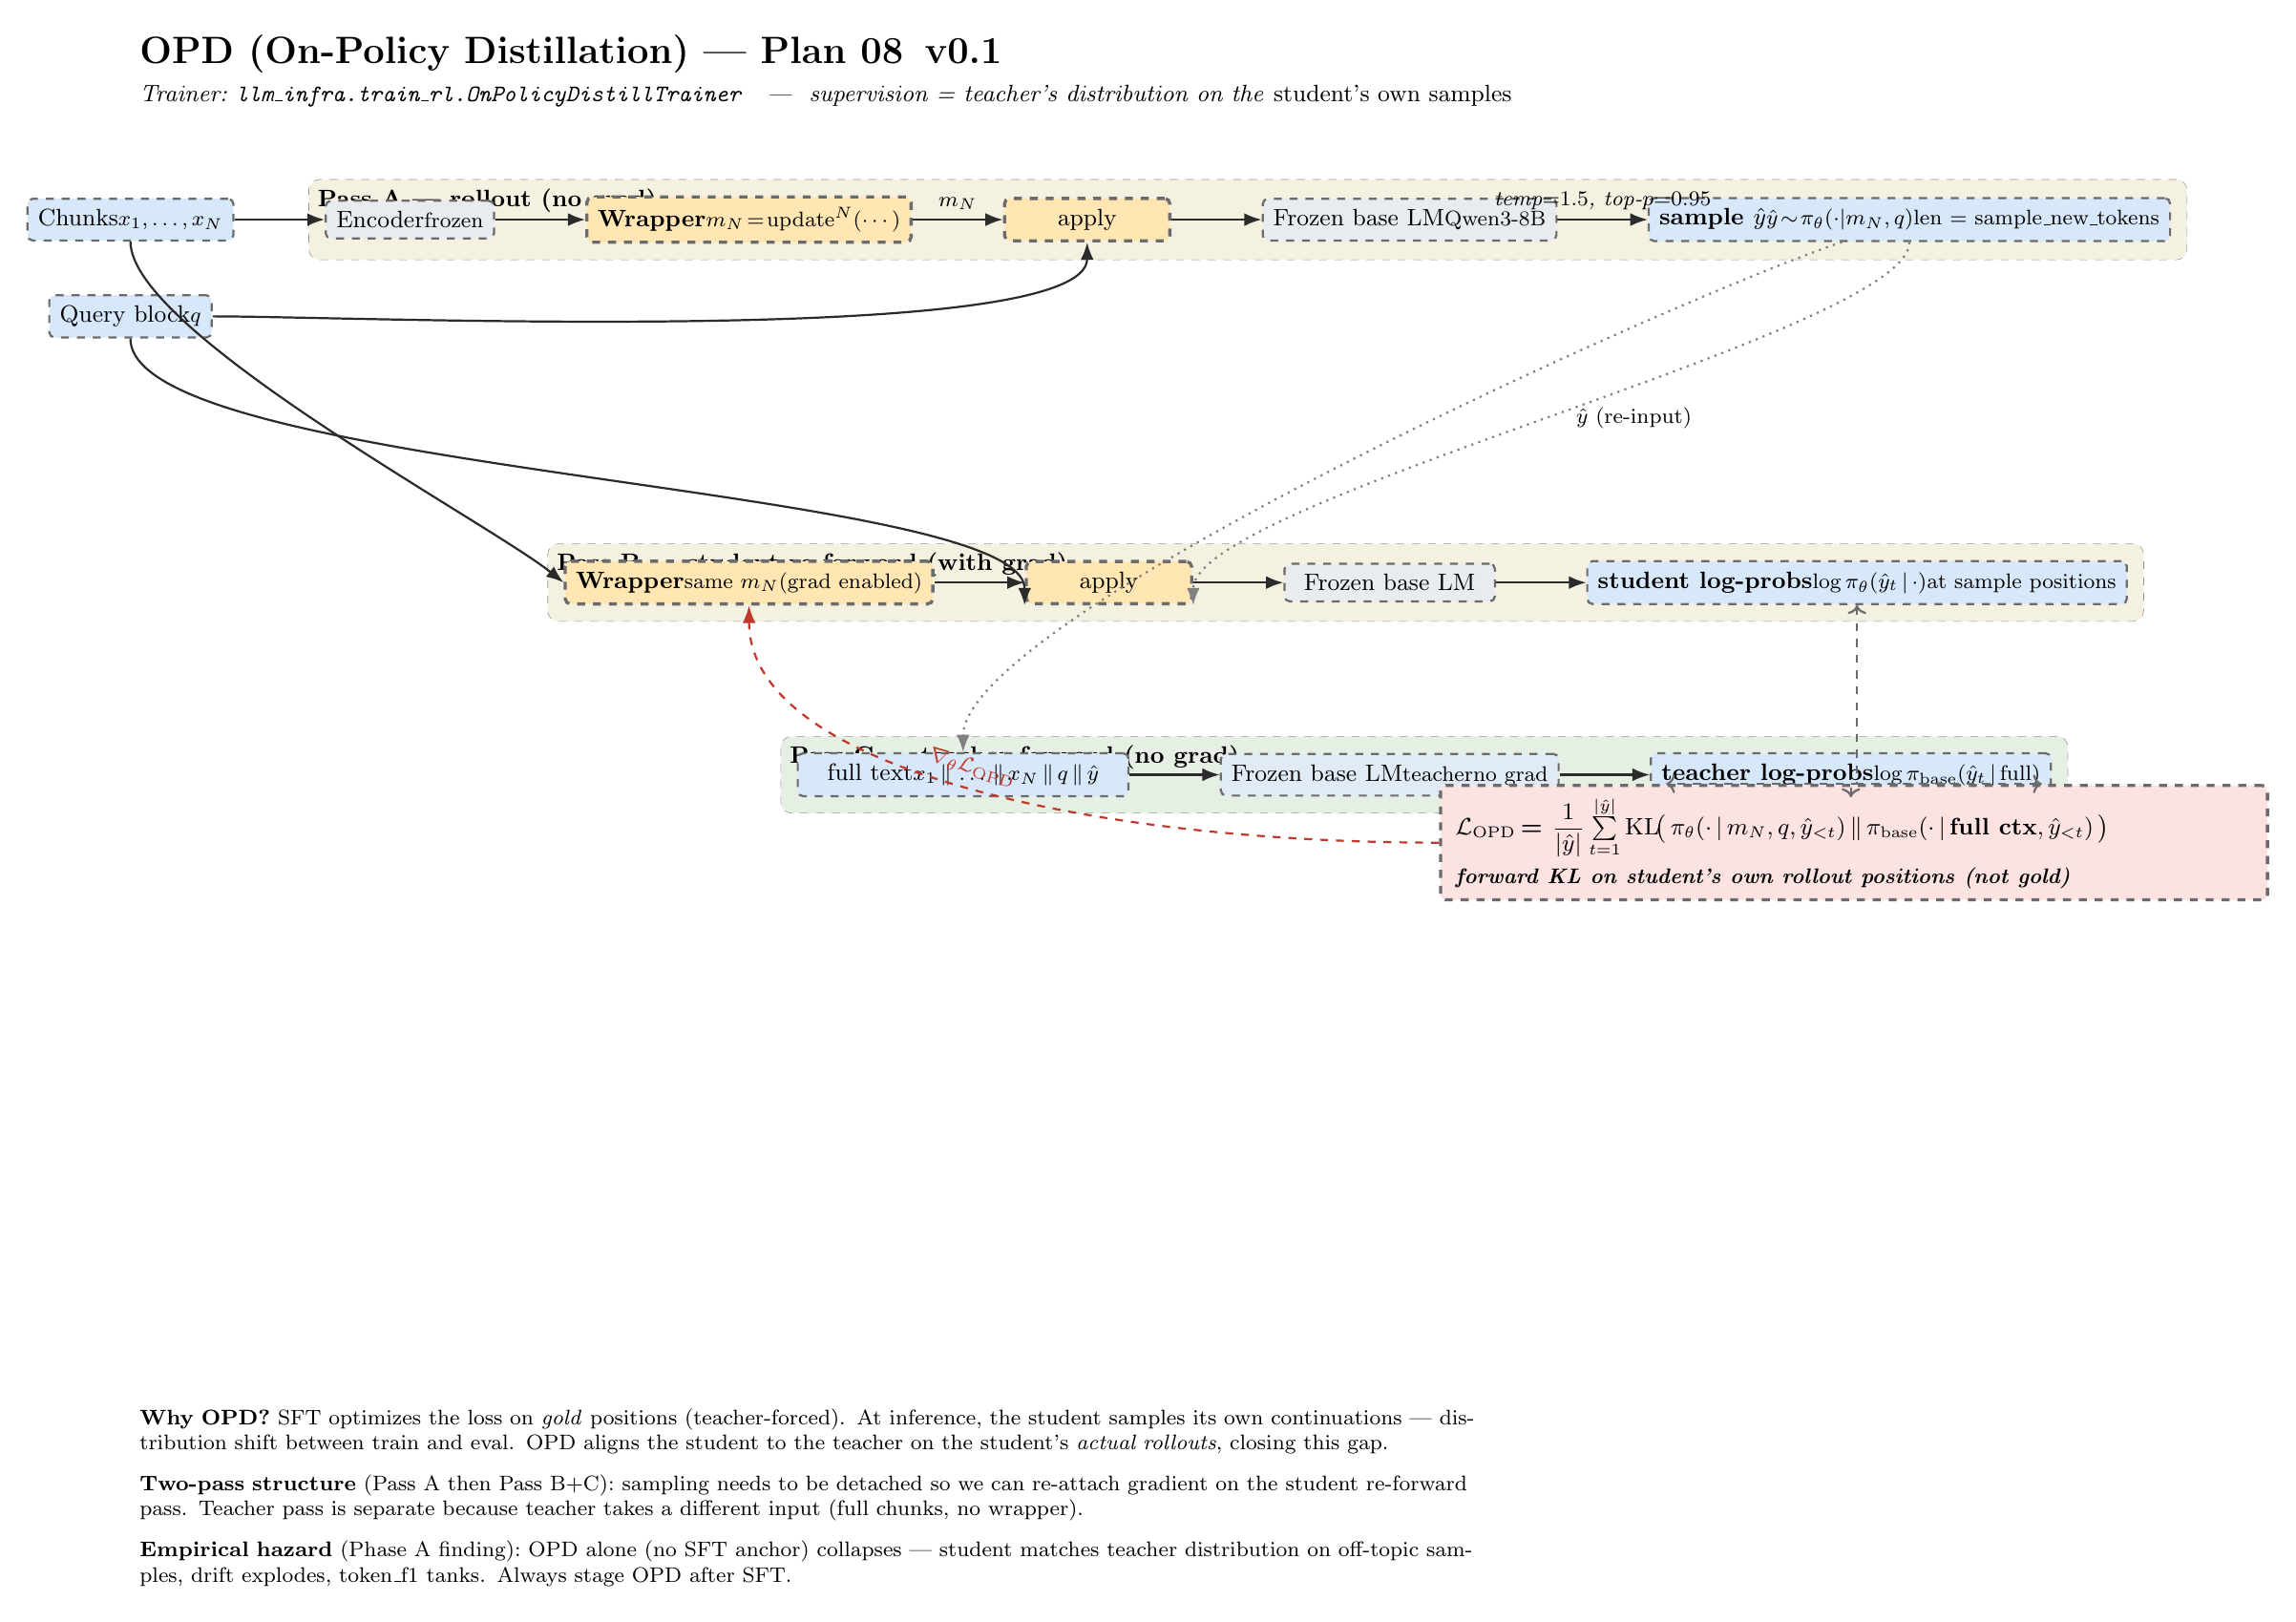
\begin{tikzpicture}[node distance=7mm and 12mm]

%% --- title -------------------------------------------------------------
\node[font=\Large\bfseries, anchor=west] (title) at (0,9.2)
  {OPD (On-Policy Distillation) — Plan 08\ \,v0.1};
\node[font=\small\itshape, anchor=west] at (0,8.65)
  {Trainer:\ \texttt{llm\_infra.train\_rl.OnPolicyDistillTrainer}\ \ \ |\ \
   supervision = teacher's distribution on the \emph{student's own samples}};

%% =====================================================================
%% Input
%% =====================================================================
\node[data] (chunks) at (0,7.0)
  {Chunks\\\footnotesize $x_1, \dots, x_N$};
\node[data, below=of chunks] (query)
  {Query block\\\footnotesize $q$};

%% =====================================================================
%% PASS A — rollout (no grad)
%% =====================================================================
\node[frozen, right=12mm of chunks] (enc) {Encoder\\\footnotesize frozen};
\node[trained, right=of enc, minimum width=42mm] (wrap)
  {\textbf{Wrapper}\\\footnotesize $m_N\!=\!\mathrm{update}^N(\cdots)$};
\node[trained, right=of wrap, minimum width=22mm] (apply)
  {apply};
\node[frozen, right=of apply, minimum width=28mm] (base)
  {Frozen base LM\\\footnotesize Qwen3-8B};
\node[data, right=of base] (sample)
  {\textbf{sample $\hat y$}\\\footnotesize $\hat y\!\sim\!\pi_\theta(\cdot|m_N,q)$\\\footnotesize len ${=}$ sample\_new\_tokens};

\draw[flow] (chunks) -- (enc);
\draw[flow] (enc) -- (wrap);
\draw[flow] (wrap) -- node[above,font=\footnotesize]{$m_N$} (apply);
\draw[flow] (query.east) .. controls +(20mm,0) and +(0,-14mm) .. (apply.south);
\draw[flow] (apply) -- (base);
\draw[flow] (base) -- node[above,font=\footnotesize\itshape]{temp${=}1.5$, top-$p{=}0.95$} (sample);

\begin{pgfonlayer}{background}
  \node[passA, fit=(enc)(wrap)(apply)(base)(sample), label={[font=\small\bfseries, anchor=north west]north west:Pass A — rollout (no grad)}] {};
\end{pgfonlayer}

%% =====================================================================
%% PASS B — student re-forward (with grad) on sampled tokens
%% =====================================================================
\node[trained, below=42mm of wrap, minimum width=42mm] (wrap2)
  {\textbf{Wrapper}\\\footnotesize same $m_N$\\\footnotesize (grad enabled)};
\node[trained, right=of wrap2, minimum width=22mm] (apply2) {apply};
\node[frozen, right=of apply2, minimum width=28mm] (base2)
  {Frozen base LM};
\node[data, right=of base2] (logp_s)
  {\textbf{student log-probs}\\\footnotesize $\log\pi_\theta(\hat y_t\,|\,\cdot)$\\\footnotesize at sample positions};

\draw[flow] (chunks.south) .. controls +(0,-12mm) and +(-10mm,8mm) .. (wrap2.west);
\draw[flow] (wrap2) -- (apply2);
\draw[flow] (query.south) .. controls +(0,-18mm) and +(0,16mm) .. (apply2.south west);
\draw[noflow] (sample.south) .. controls +(0,-12mm) and +(0,14mm) ..
   node[midway, right, font=\footnotesize, xshift=2mm]{$\hat y$ (re-input)} (apply2.south east);
\draw[flow] (apply2) -- (base2);
\draw[flow] (base2) -- (logp_s);

\begin{pgfonlayer}{background}
  \node[passA, fit=(wrap2)(apply2)(base2)(logp_s), label={[font=\small\bfseries, anchor=north west]north west:Pass B — student re-forward (with grad)}] {};
\end{pgfonlayer}

%% =====================================================================
%% PASS C — teacher forward on (chunks+query+sample), no grad
%% =====================================================================
\node[teacher, below=20mm of base2, minimum width=28mm] (base_t)
  {Frozen base LM\\\footnotesize teacher\\\footnotesize no grad};
\node[data, left=of base_t, minimum width=44mm] (cat_t)
  {full text\\\footnotesize $x_1\,\|\,\dots\,\|\,x_N\,\|\,q\,\|\,\hat y$};
\node[data, right=of base_t] (logp_t)
  {\textbf{teacher log-probs}\\\footnotesize $\log\pi_{\mathrm{base}}(\hat y_t\,|\,\text{full})$};

\draw[noflow] (sample) .. controls +(-30mm,-10mm) and +(0,18mm) .. (cat_t.north);
\draw[flow] (cat_t) -- (base_t);
\draw[flow] (base_t) -- (logp_t);

\begin{pgfonlayer}{background}
  \node[passB, fit=(cat_t)(base_t)(logp_t), label={[font=\small\bfseries, anchor=north west]north west:Pass C — teacher forward (no grad)}] {};
\end{pgfonlayer}

%% =====================================================================
%% Loss
%% =====================================================================
\node[loss, below=14mm of $(logp_s)!0.5!(logp_t)$,
      minimum width=110mm, text width=106mm] (loss)
  {\textbf{$\mathcal{L}_{\mathrm{OPD}}$\,=}\
   $\dfrac{1}{|\hat y|}\sum\limits_{t=1}^{|\hat y|}
    \mathrm{KL}\!\bigl(\,\pi_\theta(\cdot\,|\,m_N, q, \hat y_{<t})\,\Vert\,\pi_{\mathrm{base}}(\cdot\,|\,\text{full ctx}, \hat y_{<t})\,\bigr)$\\[1mm]
   \footnotesize\textit{forward KL on \textbf{student's own rollout positions} (not gold)}};

\draw[align] (logp_s) |- ($(loss.north)+(-25mm,0)$);
\draw[align] (logp_t) |- ($(loss.north)+(25mm,0)$);

%% =====================================================================
%% Gradient
%% =====================================================================
\draw[grad] (loss.west) .. controls +(-45mm,0) and +(0,-22mm) .. (wrap2.south)
  node[midway,above,font=\footnotesize\bfseries,text=gradclr,sloped]
  {$\nabla_\theta\mathcal{L}_{\mathrm{OPD}}$};

%% =====================================================================
%% Notes
%% =====================================================================
\node[font=\footnotesize, anchor=west, text width=180mm] at (0,-10.0)
  {\textbf{Why OPD?}\ SFT optimizes the loss on \emph{gold} positions (teacher-forced).
    At inference, the student samples its own continuations — distribution shift between train
    and eval. OPD aligns the student to the teacher on the student's \emph{actual rollouts},
    closing this gap.\medskip\\
   \textbf{Two-pass structure} (Pass A then Pass B+C): sampling needs to be detached so we
    can re-attach gradient on the student re-forward pass. Teacher pass is separate because
    teacher takes a different input (full chunks, no wrapper).\medskip\\
   \textbf{Empirical hazard} (Phase A finding):\ OPD alone (no SFT anchor) collapses — student
    matches teacher distribution on off-topic samples, drift explodes, token\_f1 tanks. Always
    stage OPD after SFT.};

\end{tikzpicture}
\end{document}
